%\documentclass[11pt]{article}  % for e-submission to ApJ
\documentclass[11pt]{NSF}  % for e-submission to ApJ

\usepackage[paper=letterpaper]{geometry}
\textwidth = 7.0 in
\textheight = 9.1 in
\oddsidemargin = -0.25 in
\evensidemargin = 0.25 in
\topmargin = 0.0 in
\headheight = 0.0 in
\headsep = 0.0 in
\parskip = 0.0 in
\parindent = 5.mm
\usepackage{graphicx, color, bm, amsmath, epsfig}


\usepackage{graphicx, natbib, color, bm, amsmath, epsfig}
\usepackage{wrapfig}

%paper commands, for when not using aastex
\newcommand\physrep{Phys.~Rep.}
\newcommand\fcp{Fund.~Cosmic~Phys.}
\newcommand{\pre}{Phys Rev E}
\newcommand{\apj}{ApJ}
\newcommand{\apjs}{ApJS}
\newcommand{\aj}{AJ}
\newcommand{\aap}{A\&A}
\newcommand{\mnras}{MNRAS}
\newcommand{\araa}{ARA\&A}
\newcommand{\procspie}{Proc.SPIE}
\newcommand{\pasj}{PASJ}
\newcommand{\iaucirc}{IAU Circ.}
\newcommand{\aplett}{AP Letters}
\newcommand{\aaps}{AAPS}
\newcommand{\aapr}{AAPR}
\newcommand{\nat}{Nature}
\newcommand{\apjsupp}{ApJS}
\newcommand{\pasp}{PASP}
\newcommand{\apjl}{ApJL}
\newcommand\prl{Phys.~Rev.~Lett.}
\newcommand\apss{Ap\&SS}




%%%% PUT NEW COMMANDS AND DEFINITIONS HERE %%%%
\usepackage{graphicx, natbib, color, bm, amsmath, epsfig}

%
% Hijacked and hacked from aastex.cls
%
%\def\newblock{\hskip .11em\@plus.33em\@minus.07em}%

%\newcommand\plotone[1]{%
% \typeout{Plotone included the file #1}
% \centering
% \leavevmode
% \includegraphics[width={\eps@scaling\columnwidth}]{#1}%
%}
%\newcommand\plotone[1]{
% \includegraphics[width=3.0in]{#1}%
%}
%\let\tableline=\hline
%enzo commands
\newcommand\jcompphys{J.~Comput.~Phys}
\newcommand\physfluidsa{Phys.~Fluids~A}
\newcommand\physfluids{Phys.~Fluids}
\newcommand\physlettA{Phys.~Lett.~A}
\newcommand\jfm{J.~Fluid~Mech.}
\newcommand\ccm{Comput.~Phys.~Commun.}
\newcommand\jphysique{J.~Physique~I}
\newcommand\revmodphys{Rev.~Mod.~Phys.~}

%\newcommand\aap{\ref@jnl{A\&A}}% 
%\newcommand\prb{\ref@jnl{Phys.~Rev.~B}}% 
          % Physical Review B: Solid State 


\newcommand{\ratio}{\mathcal{R}}
\newcommand{\yt}{{\tt yt}}
\newcommand{\Lmax}{\ell_{\rm max}}
\newcommand{\enzo}{{\small Enzo}}
\newcommand{\menzo}{{EnzoMHD}}
\newcommand{\Menzo}{{EnzoMHD}}
\newcommand{\zeus}{{\small ZEUS}}
\newcommand{\Lbox}{L_{\rm box}}
\newcommand{\Nroot}{N_{\rm root}}
\newcommand{\K}{\,\rm K}
\newcommand{\dave}{DaveThena}
\newcommand{\grid}{{\tt grid}}

%\newcommand{\lct}[3]{\ensuremath{\epsilon_{#1,#2,#3}}}
\newcommand{\lct}[1]{\ensuremath{\epsilon_{#1}}}
%grid location commands.
\newcommand{\iph}{i + \frac{1}{2}}
\newcommand{\imh}{i - \frac{1}{2}}
\newcommand{\jph}{j + \frac{1}{2}}
\newcommand{\jmh}{j - \frac{1}{2}}
\newcommand{\kph}{k + \frac{1}{2}}
\newcommand{\kmh}{k - \frac{1}{2}}

\newcommand{\ipmh}{i \pm \frac{1}{2}}
\newcommand{\half}{\frac{1}{2}}
\newcommand{\quart}{\frac{1}{4}}
\newcommand{\tquart}{\frac{3}{4}}

%physics commands
\newcommand{\avir}{\ensuremath{\alpha_{\rm{vir}}}}
\newcommand{\mach}{\ensuremath{\mathcal{M}}}
\newcommand{\hmag}{\ensuremath{H_{\rm{M}}}}
\newcommand{\alfmach}{\ensuremath{\mathcal{M_{\rm{A}}}}}
%\newcommand{\msun}{\ensuremath{\rm{M}_\odot}}
\newcommand{\msun}{\ensuremath{M_\odot}}
\newcommand{\lsun}{\ensuremath{L_\odot}}
\newcommand{\rsun}{\ensuremath{R_\odot}}

\def\mch{\ensuremath{M_{\rm{Ch}}}}
\def\AD{{\rm{AD}}}

%math commands
\def\rms{\ensuremath{\rm{rms}}}
\newcommand{\pts}[1]{\emph{(#1 pts)}}
\newcommand{\dbd}[2]{\frac{ \partial #1 }{ \partial #2} }
\newcommand{\ddbd}[2]{\frac{ d #1 }{ d #2} }
\newcommand{\dDbD}[2]{\frac{ \mathrm{D} #1 }{ \mathrm{D} #2} }
\newcommand{\curl}{\nabla \times}
\newcommand{\divb}{\ensuremath{\nabla \cdot {\bvec}}}
\newcommand{\divv}{\ensuremath{\nabla \cdot {\vvec}}}
\newcommand{\divbo}{$\nabla \cdot {\bf B} = 0$}
\newcommand{\intd}[1]{\int_#1^{#1 + \Delta #1} }
\newcommand{\dt}{\Delta t}
\newcommand{\dx}{\Delta x}
\newcommand{\dy}{\Delta y}
\newcommand{\dz}{\Delta z}
\newcommand{\p}[1]{#1^\prime }
\newcommand{\pp}[1]{#1^{\prime \prime} }
\newcommand{\tff}{\ensuremath{t_{\rm{ff}}}}
\newcommand{\kkmin}{\ensuremath{k/k_{\rm{min}}}}
\newcommand{\kmax}{\ensuremath{k_{\rm{max}}}}

%dcc color commands
\definecolor{orange}{rgb}{1.        ,  0.54,  0}
\newcommand{\orange}[1]{\textcolor{orange}{#1}}

\newcommand{\gtt}[1]{\textcolor{green}{{\tt#1}}}
\newcommand{\red}[1]{\textcolor{red}{#1}}
\newcommand{\yellow}[1]{\textcolor{yellow}{#1}}
\newcommand{\blue}[1]{\textcolor{blue}{#1}}
\definecolor{meta}{rgb}{0.371,0.617,0.625} %cadet blue for
                                           %non-production worthy
                                           % discussion of the work
\newcommand{\meta}[1]{\textcolor{meta}{#1}}
\newcommand{\green}[1]{\textcolor{green}{#1}}
\newcommand{\aake}[1]{\textcolor{blue}{#1}}
\newcommand{\bld}[1]{\mathbf{#1}}

\def\here{\red{notes later}}
%\newcommand{\hilite}[1]{\textcolor{red}{#1}}
%\newcommand{\hilite}[1]{#1}

%\newcommand{\bold}[1]{{\bf #1}}
%the comment maker, dc: the first one will show all comments in green, 
%the second hides them all.
%\newcommand{\dc}[1]{\textcolor{green}{#1}}
\newcommand{\dc}[1]{}
%\newcommand{\dc}[1]{#1}
%\def\bvec{\ensuremath{\vec{B}}}
%\def\vvec{\ensuremath{\vec{v}}}
\def\Bvec{\ensuremath{{\bf B}}}
\def\Jvec{\ensuremath{{\bf J}}}
\def\Avec{\ensuremath{{\bf A}}}
\def\bvec{\ensuremath{{\bf b}}}
\def\vvec{\ensuremath{{\bf v}}}
\def\uvec{\ensuremath{{\bf u}}}
\def\rvec{\ensuremath{{\bf r}}}
\def\xvec{\ensuremath{{\bf x}}}
\def\kvec{\ensuremath{{\bf k}}}
\def\Omegavec{\ensuremath{{\bf \Omega}}}
\def\omegavec{\ensuremath{{\bf \omega}}}
%\newcommand{\BlockOut}[1]{}
\newcommand{\BlockOut}[1]{#1}
\newcommand{\imp}{\ensuremath{\implies}}
\newcommand{\question}[1]{\textcolor{red}{#1}}
\definecolor{pink}{rgb}{1.        ,  0.75294118,  0.79607843}
\definecolor{maroon}{rgb}{0.69019608,  0.18823529,  0.37647059}
\newcommand{\ToRead}[1]{\textcolor{maroon}{#1}}
\newcommand{\ToReadUrgent}[1]{\textcolor{red}{#1}}
\newcommand{\HaveRead}[1]{\textcolor{black}{#1}}
\newcommand{\Old}[1]{\textcolor{blue}{#1}}
\newcommand{\Scanned}[1]{\textcolor{meta}{#1}}
\newcommand{\dccnote}[1]{}
%\newcommand{\dccnote}[1]{\textcolor{red}{#1}}
\def\nn{\nonumber}

\newcommand{\get}[1]{\textcolor{red}{#1}}
\definecolor{gray}{rgb}{0.5,0.5,0.5}
\newcommand{\gray}[1]{\textcolor{gray}{#1}}
\newcommand{\clean}[1]{\textcolor{gray}{#1}}
\newcommand{\ToDo}[1]{\textcolor{red}{#1}}
\def\etal{{\sl et al.}}

%chemistry commands
\newcommand{\Htwo}{\ensuremath{\rm{H}_2}}
\newcommand{\twelveco}{\ensuremath{^{12}\rm{CO}}}
\newcommand{\thirteenco}{\ensuremath{^{13}\rm{CO}}}

\newcommand{\mhdlabel}{{_{MHD}}}
\newcommand{\gravlabel}{{_{Grav}}}
\newcommand{\fclabel}{{_{fc}}}
\newcommand{\explabel}{{_{exp}}}
\newcommand{\sci}[1]{\ensuremath{\times {10^{#1}}}}
\newcommand{\percc}{\ensuremath{\rm{cm}^{-3}}}
\newcommand{\gcc}{\ensuremath{\rm{g}\ \rm{cm}^{-3}}}
\newcommand{\kms}{\ensuremath{\rm{km}\ \rm{s}^{-1}}}
\newcommand{\cms}{\ensuremath{\rm{cm}\ \rm{s}^{-1}}}
\newcommand{\cmperg}{\ensuremath{\rm{cm}^{2}\ \rm{g}^{-1} }}
\newcommand{\cmcmpers}{\ensuremath{\rm{cm}^2\ \rm{s}^{-1} }}
\def\muG{\ensuremath{\mu\rm{G}}}
\def\micron{\ensuremath{\mu\rm{m}}}
\def\alf{Alfv\' en}
\def\Alfvenic{Alfv\' enic}
\def\sa{super-Alfv\' enic}
\def\Sa{Super-Alfv\' enic}
\def\suba{sub-Alfv\' enic}
\def\Suba{Sub-Alfv\' enic}
\def\transa{trans-Alfv\' enic}
\def\Transa{Trans-Alfv\' enic}
\def\cs{\ensuremath{c_{\rm{s}}}}
\def\va{\ensuremath{v_{\rm{A}}}}
\def\sfrff{\ensuremath{{\rm SFR_{ff}}}}
%\def\velocity{\ensuremath{\vec{v}}}
%\def\magnetic{\ensuremath{\vec{B}}}
\def\velocity{\ensuremath{{\bf v}}}
\def\magnetic{\ensuremath{{\bf B}}}
\newcommand{\Fourier}[1]{\ensuremath{\tilde{#1}}}
\def\hfw{0.49}
\def\hw{0.49}
\def\fw{0.9}

\def\ssp{\def\baselinestretch{1.0}\large\normalsize}

\def\rhoc{\ensuremath{\rho_{\rm{c}}}}
\def\erf{\ensuremath{\rm{erf}}}


\def\SUtotal{2.9\sci{5}       }%cut from table1.
\def\tfinal{T_{\rm{final}}}
\def\suzu{\ensuremath{\rm{SU}_{\rm{zu}}}}
\def\nzones{N_{\rm{z},\ell}}
\newcommand{\Lund}{\ensuremath{\mathrm{S}}}
%\newcommand{\SUestimate}[1]{\textcolor{red}{#1}}
\newcommand{\SUestimate}[1]{#1}
\def\SUtotal{1.6\sci{5}       }                                                       
%\def\SUturb{1.8\sci{4}}
%\def\SUcore{1.2\sci{4}}
%\def\SUcmb{2.6\sci{4}}
%\def\SUgal{2.2\sci{3}}
%\def\DiskTurb{5.6\sci{3} Gb}
%\def\DiskCore{1.6\sci{5} Gb}
%\def\Diskcmb{1.7\sci{4} Gb}
%\def\Diskgal{1.1\sci{4} Gb}
%\def\StoreTotal{1.9\sci{5} Gb}
\def\nameTurbulence{\emph{turbulence}}
\def\nameTurbShort{\emph{turb}}
\def\nameCores{\emph{cores}}
\def\nameCMB{\emph{foregrounds}}
\def\nameGalaxies{\emph{galaxies}}
\def\suPerZoneUpTurbulence{\ensuremath{2.0\sci{-11}}}
\def\suPerZoneUpCores{\ensuremath{6.2\sci{-11}}}
\def\suPerZoneUpCMB{\ensuremath{6.2\sci{-11}}}
\def\suPerZoneUpGalaxies{\ensuremath{3\sci{-10}}}

\citestyle{aa}  % correct formatting for ApJ style files

\usepackage{aas_macros}
\begin{document}

\begin{centering}
\begin{LARGE}
%  Scaling Information for 
    Four Projects in Astrophysical Magnetohydrodynamics
\end{LARGE}

\renewcommand{\section}[1]{\red{#1}}
\vspace{2mm}
{\bf PI: David C. Collins} (Florida State University)

\end{centering}
\pagestyle{plain}

%\red{TO DO}
%`` Note that the proposal appears hastily put together, with typographical
%errors throughout.''
%
%``The authors neglected to provide specific information on how the runs would be
%setup. This must be included in future proposals or they may be rejected.''
%
%`` However, the most important information is missing (or at least I could not
%find it): How many cores will be used during the proposed calculations? Without
%this information the scaling plot is not very useful, and particularly the
%'effective use of resources' cannot be judged properly. ''
%
%``For now I recommend to award 50\% of the request, which will allow the group to
%start with the parameter study. Scarce resources will also encourage the group
%to prune the parameter list after initial results roll in. ''
%\tableofcontents
%\input{abstract}       %dcc todo 2022
\section{Introduction}
\label{sec.intro}

We are requesting \SUtotal\ SUs on Stampede 2 for the period beginning June 1,
2022.  This allocation will support four projects involving astrophysical
magnetic fields and turbulence.  The first project  (\nameCMB) examines the polarized signal
produced by the interstellar medium, which is in the foreground of our understanding of
the distant cosmic microwave background (CMB). The second project (\nameTurbulence) explores analytical
formulae we have developed for isothermal turbulence, which is relevant for many
astrophysical processes, among them the formation of stars.
  The third project (\nameCores) examines fractal structures in star forming clouds. The fourth project (\nameGalaxies)
simulates entire galaxies, in order to understand the growth of the magnetic
field, and the spatial distribution of magnetic fields for CMB foreground
removal.
This research is supported by two NSF grants.  The first two projects
(\nameTurbulence\ and \nameCores)  
are
supported by NSF AST-1616026, and the third (\nameCMB) is supported by 
NSF AST-2009870.
We are hopeful that the \nameGalaxies\ project will be funded by a pending
proposal.

These projects support three graduate students.  Luz Jimenez Vela is working on
the \nameCores\ project; Branislav Rabatin is working on the \nameTurbulence\
and \nameCMB\ projects; and Jacob Strack is working on the \nameGalaxies\
project.


Table \ref{table1} shows the cost for each project in SUs, as well as the disk
usage, physics packages, number of simulations to be run, and number of nodes to
be used.  64 cores per node will be used for all runs.  Also included is the
storage need for our existing archive of data, much of which is still generating
publications.
Two projects are fixed resolution driven turbulence (\nameTurbulence and \nameCMB), and two use
more expensive gravity and adaptive mesh refinement (\nameCores\ and
\nameGalaxies). In Section \ref{sec.method} we
describe the computational tools to be used.  
We motivate each project and describe the simulations to be
run in Section
\ref{sec.background}.  In Section \ref{sec.plan} we
give the projected cost  and disk usage of these simulations.

    %dcc todo 2022
\def\SUtotal{4.3\sci{4}       }                                                                       
\begin{table}[h] \begin{center} \caption{Summary of allocation request. The total node hours and disk usage
are in the first two columns, broken down by project. The physics packages used in
eash project  determine the cost and scalability. $N_{sim}$ is the number of simulations
in the suite, some of which may run concurrently.
$N_N$, is in the number of nodes to be used.  64 cores per node will be used
for all simulations.
}

 \label{table1}                                                                                       
\begin{tabular}{l               r               r               r               r               r      }
    Name       &Node Hours       &    Disk       & Physics       &$N_{sim}$       &   $N_N$     \\
  \hline                                                                                       
\nameCMB       &1.5\sci{4}       &9.0\sci{3}       &Driven Turbulence       &       4       &      64     \\
\nameTurbulence       &2.4\sci{4}       &4.0\sci{3}       &Driven Turbulence       &       5       &      64     \\
\nameCores       &1.0\sci{3}       &2.0\sci{4}       &Gravity+AMR       &       3       &       8     \\
\nameGalaxies       &2.9\sci{3}       &1.1\sci{3}       &Gravity+AMR       &       2       &       8     \\
 Archive       &      --       &7.0\sci{4}       &               &               &             \\
  \hline                                                                                       
               &4.3\sci{4}       &1.0\sci{5}       &               &               &             \\
\end{tabular}                                                                                       
\end{center}                                                                                       
\end{table}                                                                                        
\section{Scientific Background}
\label{sec.background}

The common thread among these projects is turbulence.  We discuss the aspects of
turbulence that apply to all of our projects in Section
\ref{sec.turbulence}.  We discuss the relevance of each project and the simulations to be run in
the sections that follow.
We present the \nameCMB\ project in Section
\ref{sec.back_foregrounds}, the \nameTurbulence\ project in Section
\ref{sec.back_turb}, the \nameCores\ project in \ref{sec.back_cores}, and
finally the \nameGalaxies\ project in \ref{sec.back_galaxies}.


\subsection{Background: Turbulence Basics}
\label{sec.turbulence}
Turbulence underpins all of the projects in this proposal, the first two most
notably.  Here we describe the aspects of a turbulent system that impact the
design of our simulations, the excellent work of \citet{Frisch95} has more
details.

In a turbulent system, energy is injected at a scale, $L_{driving}$.  By way of
fluid instabilities, the energy cascades to smaller and smaller scales until
molecular interactions dissipate the energy at a scale $L_{diss}$.  The energy
spectrum 
behaves like a powerlaw, $E(k)=k^{a}$.  For incompressible fluid turbulence,
$a=-5/3$, but that exponent varies with the inclusion of supersonic
(compressible) flow and magnetic fields.  The region between
$L_{driving}$ and $L_{diss}$, where the powerlaw is valid, is referred to as
the \emph{inertial range}.  Here, the nonlinear inertial terms in the
Navier-Stokes equation dominates over the dissipation terms, and it is the
behavior of the nonlinear terms that we wish to explore.  $L_{driving}$ is set
by the boundary of the simulation. $L_{diss}$ is set by details of the
solver and the energy of the flow.  Thus, for a given driving energy, the only
way to increase the size of the inertial range is with resolution.  The
inclusion of magnetic fields only shrinks the inertial range and makes the
problem harder.

At a resolution of $256^3$, the driving scale and dissipation scale overlap, and
there is not much inertial range to work with.  At $512^3$, an inertial range
appears, but it is small, and determining the actual powerlaw portion of the
spectrum is error-prone.  This will be demonstrated in Section
\ref{sec.back_foregrounds}.  At $1024^3$, a reasonable powerlaw appears even for
magnetized simulations.  Further increase of the resolution is desirable, but
the cost scales like the number of zones on a side to the fourth power, while
the size of the inertial range is only linear.  Increases in resolution to
$2048^3$ and beyond is possible and desirable, but also quite costly in terms of
total $SU$, disk, and human time.  This will be explored if the results of the
current proposal indicate it is necessary.  

Turbulence is a chaotic process, and must be handled statistically.  A single
snapshot from a turbulent box is largely random, the true nature must be
averaged over a window of time.  Additionally, we focus on fully developed
turbulence, which takes some simulation time to develop. Thus we run our
simulations for a period of time to develop the turbulence, and a period of time
for statistical averaging.  This is discussed in detail in the next two
sections.

For the \nameCMB\ and \nameTurbulence\ simulations, we will use a resolution of $1024^3$ to
obtain inertial ranges that are well defined.  For the \nameCores\ suite, we
will use a root grid of $512^3$ to offset the cost of 4 levels of AMR and
gravity.  The
\nameGalaxies\ will use a root grid of $256^3$ and 8 levels of AMR, and
sacrifices well resolved turbulence for spatial dynamic range.  Properly
resolving the turbulence in the galaxy as well as the circumgalactic media is
presently impossible.  

Simulation purpose and design will be described further in the next
sections.



\begin{figure} \begin{center}
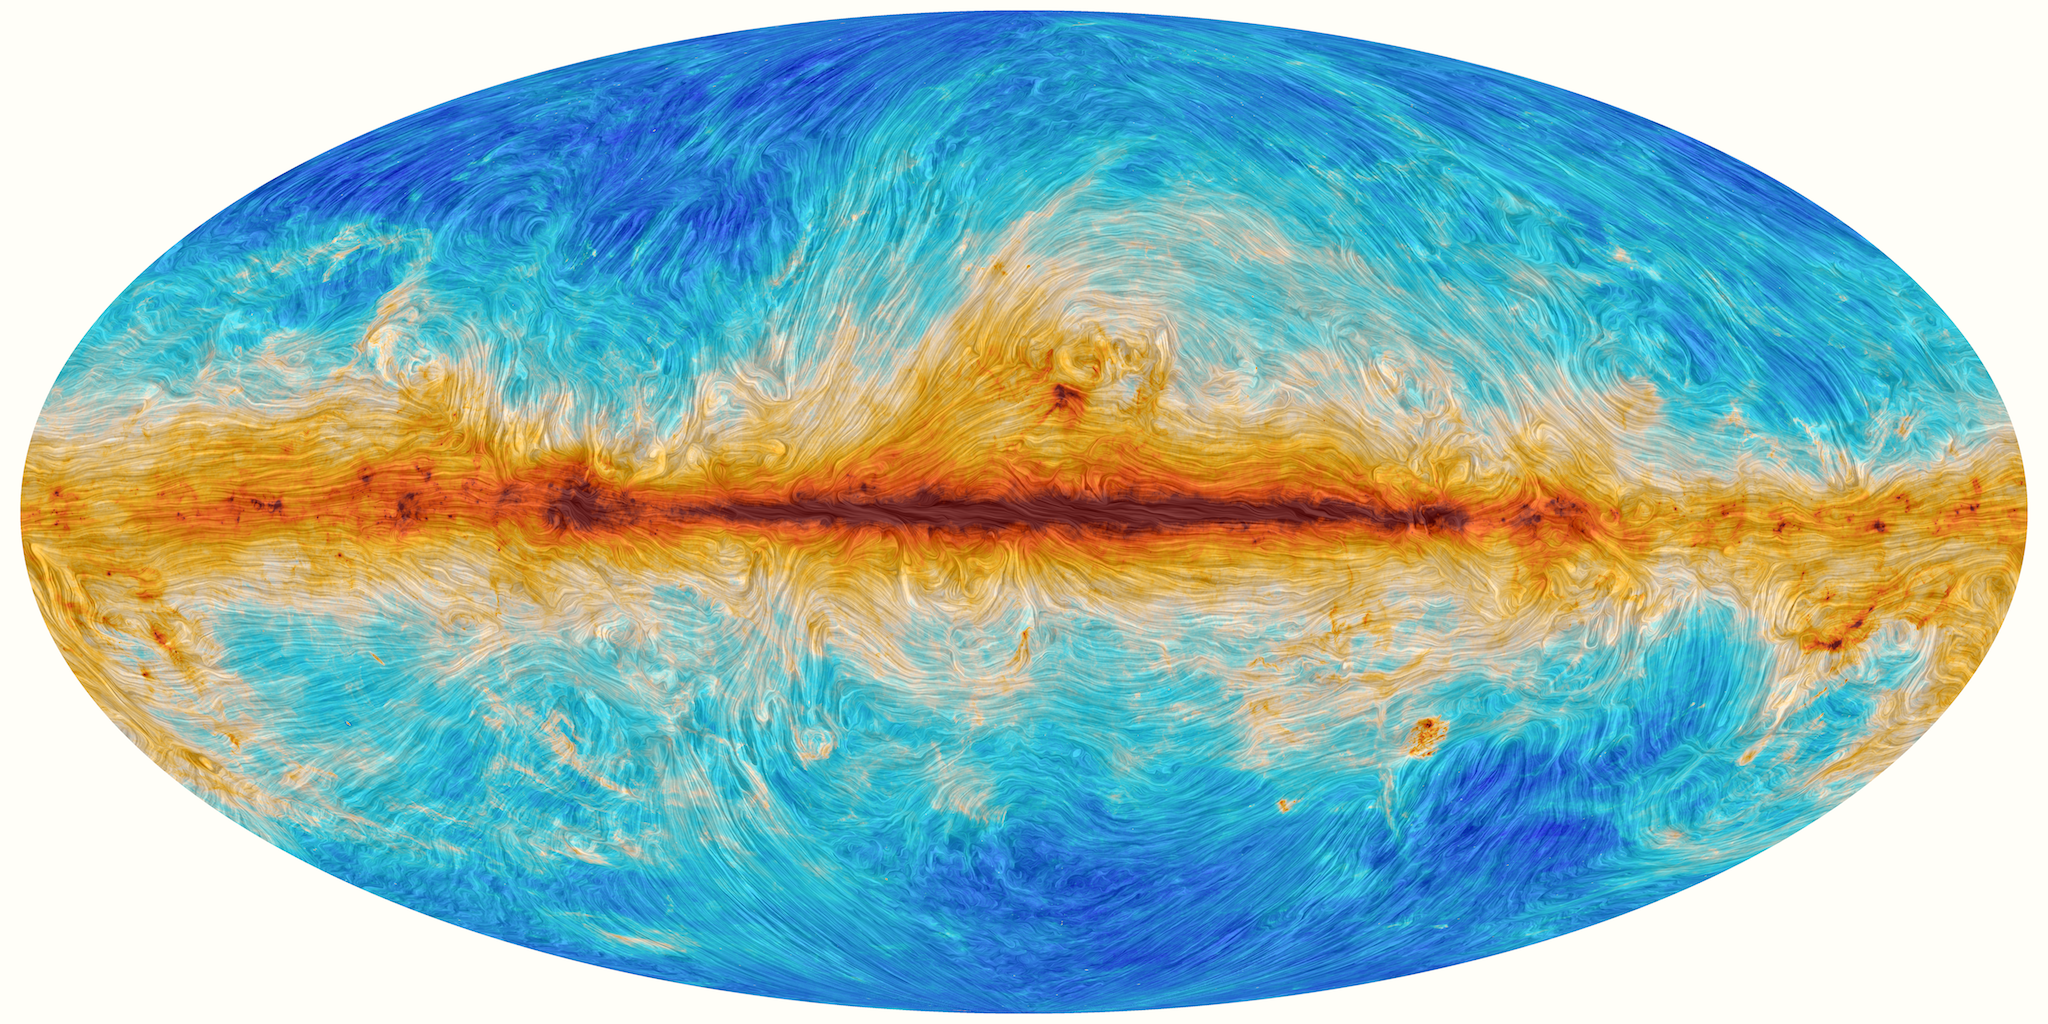
\includegraphics[width=0.55\textwidth]{figs/2015_353GHz_B-field.png}
%\includegraphics[width=0.42\textwidth]{figs/ClEE_y_12panel_average.pdf}
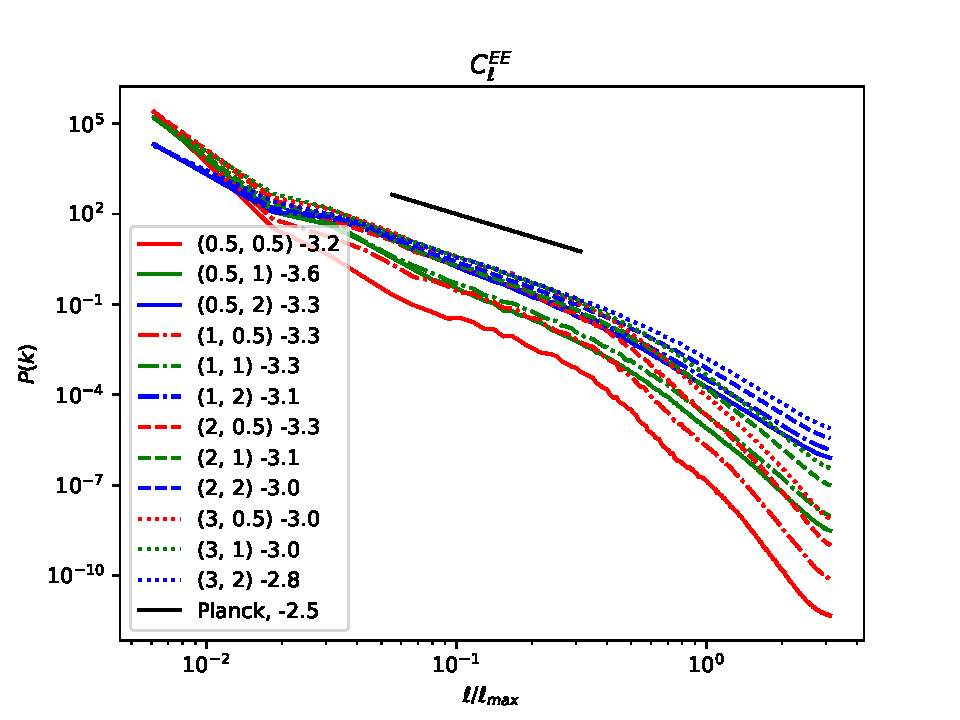
\includegraphics[width=0.42\textwidth]{figs/alpha_TEB.pdf}
\caption[ ]{\emph{(Left)} The large scale magnetic field of the galaxy as seen by the Planck
satellite. The color field shows dust emission at 353GHz.  The image is smeared
along the direction of the magnetic field \citep{PlanckXIX15}.  The \nameCMB\
project aims to remove this signal from the CMB, while the \nameGalaxies\
project aims to understand its origin. \emph{(Right)} The power spectrum of the
polarization showing $E-$mode power vs. wavenumber for a preliminary suite of
simulations.}
\label{fig.planck} \end{center} \end{figure}

\subsection{Background: CMB Foregrounds}
\label{sec.back_foregrounds}
The cosmic microwave background (CMB) is the light leftover from the creation of
the universe.  It has taught us a considerable amount about the structure,
history, and future of the
universe.  To learn more from it, we must understand its polarization.  To see
the polarization of the CMB, we must first understand the polarization of the
interstellar medium (ISM), which is much brighter and in the way.  This project
will perform simulations of driven magnetized turbulence, and compare the
filamentary structure found with an analytic model of the CMB polarization
developed by \citet{Huffenberger20}.  We will
motivate this project in Section \ref{subsec.cmb_motivate}, and describe the
simulations we will perform in Section \ref{subsec.cmb_sims}

\subsubsection{Motivation: \nameCMB}
\label{subsec.cmb_motivate}

When the universe was very young, it was very small, and also very hot.  So hot
that everything was ionized.  Sound waves generated by the big bang travel through
the universe, causing temperature fluctuations.  Once the universe cooled
enough, the electrons and protons combined to make the first Hydrogen.  After
this time, photons can travel great distances without running into an electron.
These photons are the CMB.  It is an extremely uniform 2.7K black body.  Small
($\mu K$) fluctuations in this temperature have been studied extensively by
satellites such as Planck \citep{Planck2018VI20}. These fluctuations have answered many
questions about the content and eventual fate of the universe.  But there are
still open questions.

Why is the CMB a single temperature?  The
universe is very large, and one side of the observable universe has never been
in contact with the other.  Given the expansion of the universe, one would
expect significant fluctuations in temperature on the angular size of the full moon on the sky.
One possible answer is an extremely rapid
\emph{inflation} of the universe, where the universe expands from the size of a
proton to the size of the solar system within the first $10^{-16}$s.  This is
different from the \emph{expansion} of the universe, which has been well
established and a much more leisurely pace.  Such a
rapid event would allow different patches of the universe to be at the same
temperature very early on.  
It is also extraordinarily violent, would leave a sea of gravitational waves.  These gravitational
waves, being quadrupolar in nature, imprint a polarization on the CMB. To detect
this polarization is to witness the violent birth of the Universe.

Unfortunately (for observing the CMB) the Galaxy we live in is filled with dust,
which gives a polarized signal in the same frequency range as the polarized CMB.
This dust, which includes iron and magnesium, lines up perpendicular to the magnetic
field in the galaxy, not unlike iron filings around a bar magnet.  These aligned
grains radiate polarized thermal radiation in the microwave and infrared, and so
the dust polarization is perpendicular to the magnetic field.  This
polarized signal is much brighter than the polarization in the CMB, so it must be
removed.  In order to remove it, we must understand the statistical properties
of the turbulent interstellar medium of the Galaxy. 

The polarization vector of a photon is the given by orientation of its electric field.  This is
a quantity that depends on the orientation of the camera observing it, which is
difficult to use since the camera must point over the whole sky.  We define two
rotationally invariant quantities, $E-$mode and $B-$mode, which are the
parity-even and parity-odd versions of the polarization vector.  Briefly,
$E-$mode is polarization at either 90 or 45 degrees to filamentary structure,
and $B-$mode is polarization that is at oblique angles to filaments.  More
details can be found in \citet{Rotti19}.  

The Planck satellite \citep{PlanckXIX15} measured the galactic polarization, and the result can be
seen in Figure \ref{fig.planck}.  The left panel shows the 353 GHz dust emission in color,
and the image is smeared along the direction of the magnetic field at every
point.  The right panel shows the power spectrum of the polarization from
simulations (colored lines) and Planck (black line).   This plot show
$C_\ell^{EE}$, the amplitude in $E-$mode power, vs wavenumber $\ell$.
It is found \citep{PlanckXIX15} that both quantities are
distributed over all scales in a power-law fashion, with $E \propto
\ell^{-2.5}$.
$B$ has a similar exponent but half the
amplitude.  

The colored lines in Figure \ref{fig.planck} are the results of a suite of MHD
simulations to be published in Stalpes et al 2022 (in prep).  This was a suite
of magnetized turbulence simulations at various r.m.s velocities and magnetic
field strengths at a resolution of $512^3$ performed on \emph{Stampede2}.  The
simulations were parameterized by the sonic Mach number, $\mach=v/c_s$, the r.m.s.
velocity relative to the speed of sound, $c_s$; and the \alf\ Mach number,
$\alfmach=v/c_A$, the
r.m.s velocity relative to the speed of magnetic waves, $c_A$.  These are seen
in the legend of the figure, along with the powerlaw exponent of the line.  Two things are
of note.  First, the slopes are all steeper than that found by Planck.  And
second, most notably the bottom red line, is the poor linear quality of the
resulting spectra.  These shortcomings are the result of inadequate resolution,
as discussed in Section \ref{sec.turbulence}.


\subsubsection{Simulations: \nameCMB}
\label{subsec.cmb_sims}

Our previous suite of simulations (Stalpes et al 2022, in prep) was run at a
resolution of  $512^3$, which is insufficient to match the behavior of the sky.
The current simulations will double the size of the inertial range by doubling
the resolution to $1024^3$, and target parameter space suggested by that
parameter suite.  In this case more resolution is better without
bound, as the sky we are trying to match has an astronomical separation of scales. However, doubling
the inertial range increases the cost by a factor of at least 16, so while
higher resolution is possible, is is not warranted at this time.

The turbulence in our simulations is created by way of large scale forcing, in
which energy is added to the gas at every time step at the largest scale, in a
manner that keeps the injection rate constant \citep{MacLow99, Schmidt09}.  This is
continued for 5 dynamical times, $t_{dyn}=L/V$, where $L$ is the size of the
pattern and $V$ is the r.m.s. Mach number of the flow.  The first $2 t_{dyn}$
are used to establish a steady state, within this window of time the flow is
chaotic and the spectra fluctuate wildly.  We then run for an additional $3 t_{dyn}$ to build statistics, and
average the power spectra over this window.  This gives us three statistically
independent spectra to average.  Again, more is better, three is the minimum.  

Our results from Stalpes et al (2022) indicated that an r.m.s. Mach number of 5
is necessary to reproduce the observed spectra.  We will run a suite of four
simulations with (\mach, \alfmach) = (1,1),(1,5),(5,1),(5,5).  This will allow
us to bracket the ranges of parameters the ISM experiences.



\begin{figure} \begin{center}
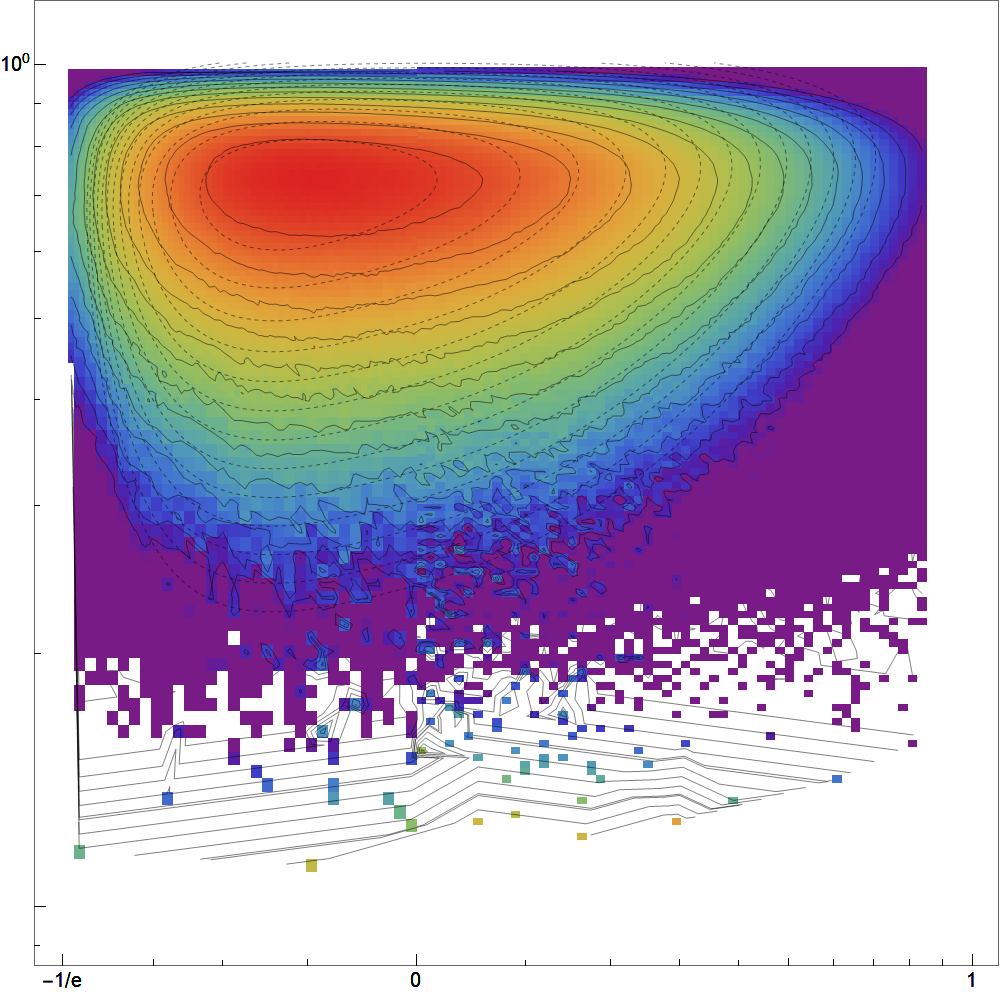
\includegraphics[width=0.32\textwidth]{figs/mach5_contours_comparison_V_MCMC.png}
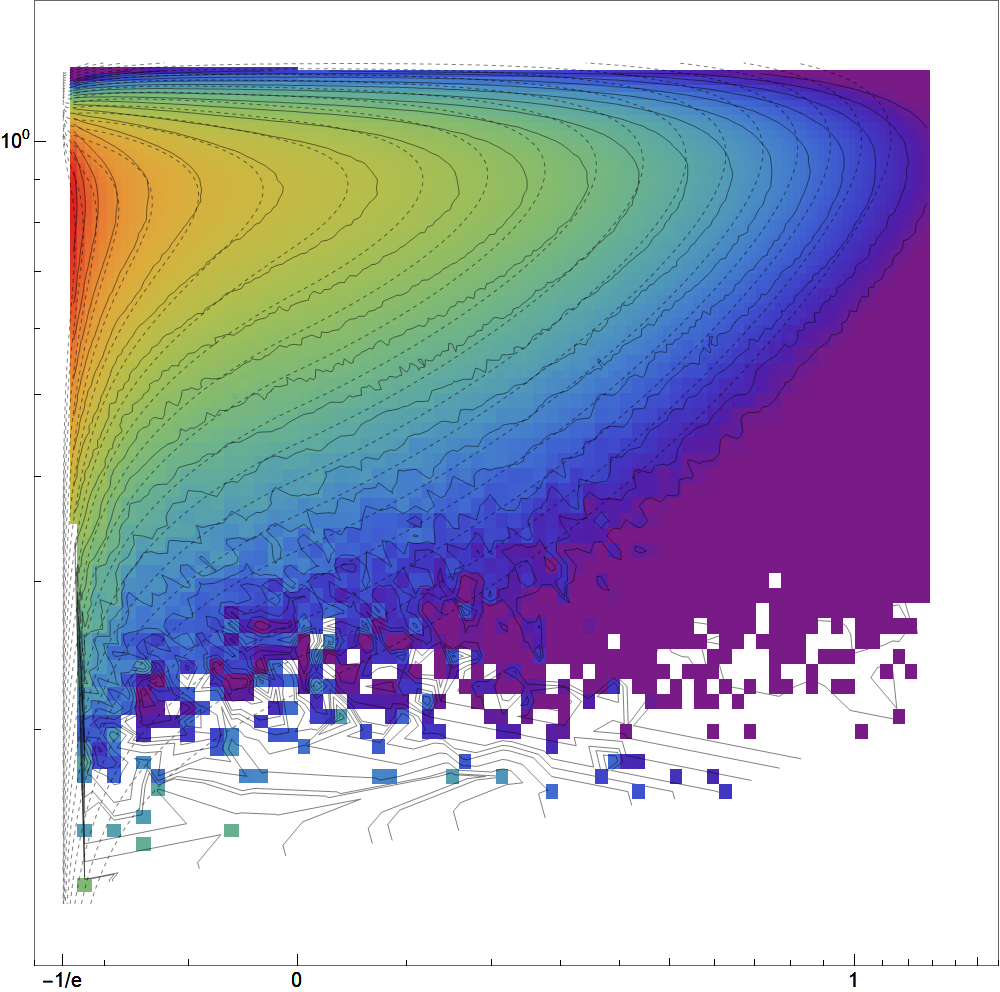
\includegraphics[width=0.32\textwidth]{figs/mach10_contours_comparison_V_MCMC.png}
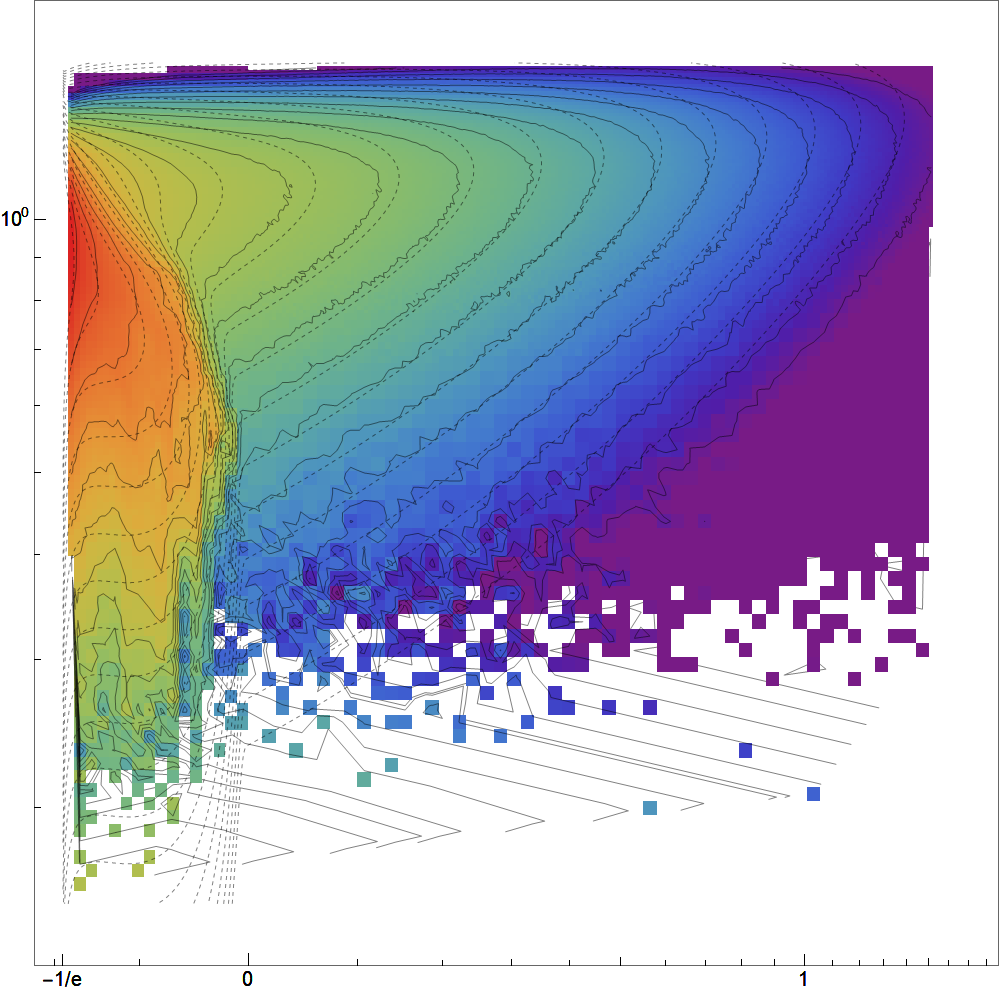
\includegraphics[width=0.32\textwidth]{figs/mach20_contours_comparison_V_MCMC.png}
\caption[ ]{The joint distribution between thermal energy, $E_T$ (horizontal), and kinetic
energy $E_K$ (vertical). Color shows the PDF computed from low resolution simulations, and ranges between 0 (purple) and 1
(red).  The thermal energy develops a low $E_T$ wall as well as a high $E_T$
wing as the Mach number increases.  Dashed lines are our analytic estimate,
which is good but has differences that are likely due to resolution. }
\label{fig.energy} \end{center} \end{figure}

\subsection{Background: Turbulent Energy PDFs}
\label{sec.back_turb}
Turbulence is ubiquitous in astrophysical processes.  We have developed analytic
predictions for the distribution of energies in isothermal turbulence, both
supersonic and subsonic. These simulations will verify our analytic predictions,
and examine if deviations seen in preliminary studies are due to lack of
resolution or interesting physics.
We provide the background for the \nameTurbulence\ project in Section
\ref{subsec.turb_motivate},
and motivate the simulations that support this study in Section
\ref{subsec.turb_sims}.


\subsubsection{Motivation: \nameTurbulence}
\label{subsec.turb_motivate}

The interstellar medium (ISM) is the gas between stars in the galaxy.  It cools
very effectively, so can be treated as isothermal \citep{Krumholz14}.  The ISM is also turbulent, with supersonic shocks driven by supernovae
causing supersonic turbulence throughout the interstellar medium
\citep{Elmegreen04}.  This
turbulence impacts the formation of stars (see Section \ref{sec.back_cores}) and
causes a polarized screen that is blocking our view of the light from the big bang (see
Section \ref{sec.back_foregrounds}), among many other effects
\citep{Elmegreen04}. It is also interesting in its own right.  We have developed
analytic formulae for the probability density function (PDF) of internal energy
and kinetic energy, as well as their joint distribution.  In this project we
will verify these formulae with high resolution simulations.

Supersonic turbulence is compressible, and the distribution of density
fluctuations is described by a log normal, i.e. the log of density is
distributed as a Gaussian \citep{Vazquez-Semadeni94}.  The distribution of velocity is roughly Maxwellian,
i.e. each of the three velocity components is a Gaussian, and added in quadrature the
distribution is Maxwellian.  
We have recently found analytic distributions for the internal energy and
kinetic energy, as well as their joint
distribution.   (Rabatin et al 2022, in prep). Kinetic energy is defined in the familiar way, $E_K=\half \rho
v^2$.  Internal energy is defined as $E_T= c_s^2 \rho \ln \rho/\rho_0$, where
$c_s$ is the sound speed and $\rho_0$ is the mean density \citep{Banerjee18}.  The joint
distribution of these two quantities can be seen in Figure \ref{fig.energy},
along with our analytic prediction (dotted lines).
Each panel shows the joint PDF of $E_K$ and $E_T$;  the color field shows the
PDF derived from data; the solid lines show logarithmically spaced contours of
the data; the dashed lines show the theoretical prediction.  The first panel is
subsonic, with $\mach=0.5$, the middle has $\mach=1$, and the third panel is
slightly supersonic, with $\mach=2$.  Significant changes in the behavior of the
distribution, with high $K_E$ gas developing along side high $E_T$ gas, are both
predicted by the analytical dashed lines and seen in the data.

Our preliminary simulations were run with a modest resolution of $256^3$.  This
is enough to find reasonable agreement, but imperfect. This can be seen most
easily in the first panel of Figure \ref{fig.energy}, by examining the center
most (red) contours. The solid line shows simulation, while the dashed line
shows theory, which clearly agrees, but only approximately.  This lack of
agreement can be one of several things, the first to examine is numerical
resolution.  With insufficient resolution, energy is transferred from large to
small scales faster than would be natural, which could be why we have mediocre
agreement in our predicted theory.  

\subsubsection{Simulations: \nameTurbulence}
\label{subsec.turb_sims}

The proposed simulations will quadruple this
resolution to $1024^3$.  Owing to the substantial evolution with Mach number, we
will run some subsonic cases (\mach=0.5, 1.0) and some moderate and highly
supersonic cases (\mach=2,4,7).  The turbulence is produced by adding a random
velocity component to the field in a manner that slowly evolves over time
\citep{Schmidt09}.  The simulations are run for $5 t_{dyn} = 0.5/\mach$, the
dynamical time is the time it takes for the forcing pattern (half the box
length) to cross the box.  Running for $5 t_{dyn}$ allows the turbulence to be
fully developed and statistically well sampled.  These are dimensionless physics
studies, so the box size and sound speed are unity.



\begin{figure} \begin{center}
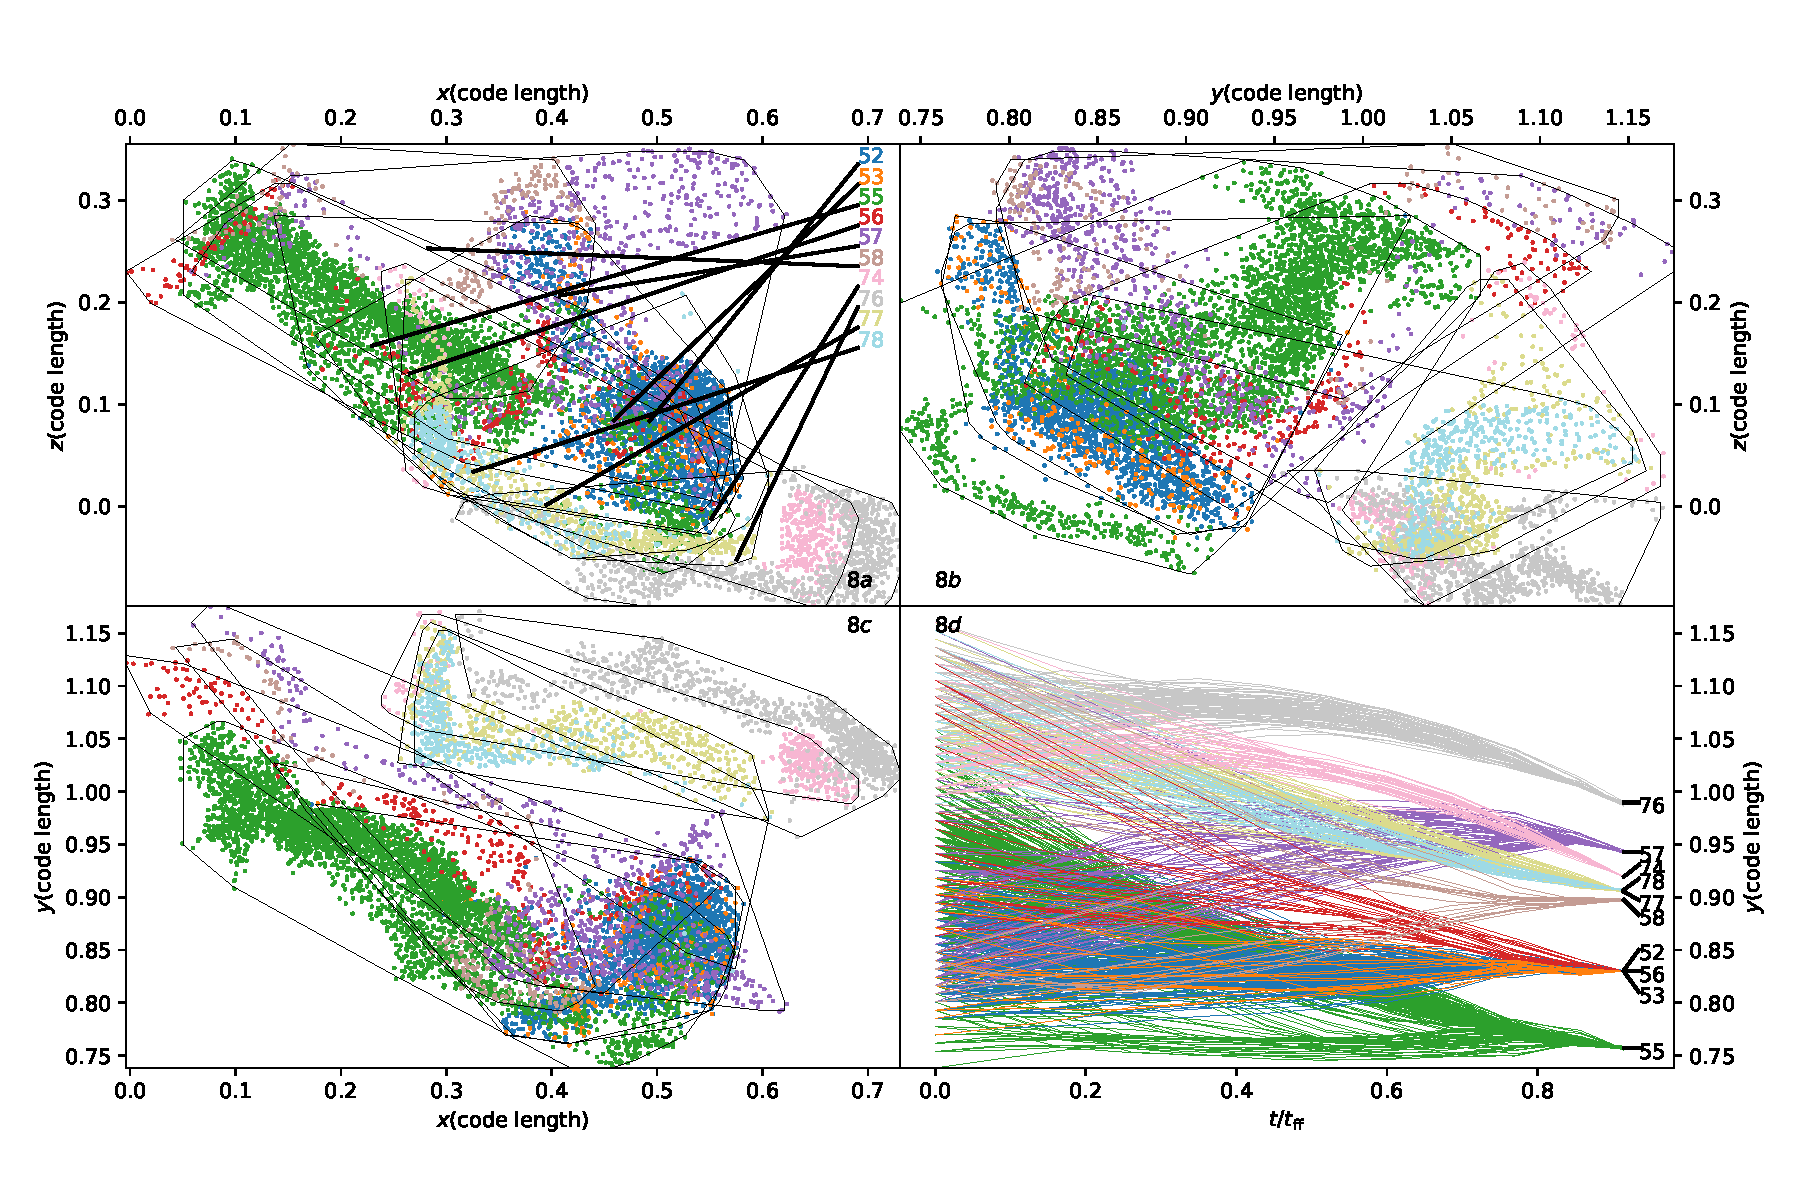
\includegraphics[width=\textwidth]{figs/overlap_hair_u603_S01.png}
\caption[ ]{The initial phase of star formation for several different cores.  These particles, seen in three
projections and one time series, all form cores by the end of the simulation,
but begin as a series of overlaping fractals}
\label{fig.cores} \end{center} \end{figure}

\subsection{Background: Star Formation}
\label{sec.back_cores}

The formation of stars is filled with filamentary, fractal structures
\citep{Andre14}.  The
\nameCores\ project will study the behavior of collapsing gas as it transitions
from fractal structures to form dense prestellar cores.  We will motivate the
study in Section \ref{subsec.cores_motivate}, and describe the simulations
in \ref{subsec.cores_sims}.


\subsubsection{Motivation: \nameCores}
\label{subsec.cores_motivate}
The formation of stars is one of the most important processes in astrophysics,
as stars provide most of the light we see in the night sky, and they produce the
energy and metal
that dictates the structure and composition of a galaxy.  
A \emph{prestellar core} is a knot of dense gas
formed by gravity in a molecular cloud, which will ultimately form a star.  The
formation of these cores is one of the more difficult puzzles in star formation,
as it is fundamentally dictated by chaotic dynamics of the turbulence in the
cloud.  This is the focus of the \nameCores\ project.

One of our previous studies (Collins et al 2022, in prep) examined the collapse of a molecular cloud by
including semi-Lagrangian tracer particles that follow the flow.  The particles
that are found in dense cores at the end of the simulation are then followed
backwards in time to 
to examine the \emph{preimage} of the gas, before it collapses.  This will allow
us to better constrain star formation models.  

One of the curious findings is the fractal nature of the preimage gas.  We find
that gas from distinct cores at the end of the simulation begins life mixed with
one another in a fractal manner. This can be seen in Figure
\ref{fig.cores}, which shows the overlap of a collection of preimages at the
beginning of the simulation in the first 3 panels, and the
collapse to form dense cores in the fourth.  The length scale in the first three panels translates to
roughly 2 pc in size.  These panels show the overlap and fractal, filamentary nature of
the gas before it collapses.  The
last panel shows the un-mixing of the gas as it collapses in time.

\subsubsection{Simulations: \nameCores}
\label{subsec.cores_sims}

The simulation presented in Figure \ref{fig.cores} was one of a suite of three
simulations with varied magnetic field strength.  We began with fully developed
turbulence, and then added tracer particles and turned on gravity and AMR.  These simulations were
relatively low resolution as we developed the analysis techniques and learned
about extended nature of the primage gas. Our proposed simulations will greatly improve the resolution
to explore if these structures are in fact fractal, or a result of low
resolution. 
The target simulations will have $512^3$ root grid and 4 levels of
AMR, and $1024^3$ particles.  This resolution strategy is a compromise between
a large root grid to resolve the turbulence and deep AMR to capture the cores.  

The size of the box is 5 pc, and the r.m.s. Mach number is 9.  They
will begin from existing simulation data.  

The proposed suite of three simulations will mirror the magnetic field strengths
of the preliminary studies.  The simulations will be similar to those presented
in \citep{Collins12}, but with tracer particles and sinks.
It will run for a total of one free-fall time, where $t_{ff}=(G
\rho)^{-1/2}=1$Myr (G is the gravitational constant and $\rho$ is the mean
density of the box).  Beyond this time, feedback from young stars begins and
alters the structure of the cloud, which is beyond the scope of this study. 




\subsection{Background: Galaxies}
\label{sec.back_galaxies}
The \nameGalaxies\ project will simulate magnetic field amplification in Milky
Way sized galaxies.
The Galactic magnetic field can be seen in Figure \ref{fig.planck}.  This figure
shows an all-sky projection of dust in the galaxy, as seen by the 353 GHz camera
on Planck.  The image is smeared along the direction of
the magnetic field, which is measured by way of the polarization of the signal.  Our goal in the \nameGalaxies\ project is to understand the
origin of this magnetic field.   We will We will discuss the background in Section
\ref{subsec.galaxies_motivate}, and describe the simulations we will perform in
Section \ref{subsec.galaxies_sims}

\subsubsection{Motivation: \nameGalaxies}
\label{subsec.galaxies_motivate}

The Milky Way has a large scale magnetic
field of roughly $\sim 5 \mu$G, about 200,000 time weaker than a refrigerator
magnet, but spanning the entire galaxy.   In the previous project, \nameCMB, the
goal is to study the properties of the field with high resolution, while in
the \nameGalaxies\ project the goal is to study the origin of this field.

The origin of this magnetic field is an open question.  There are presently two
known \emph{dynamos}, that is mechanisms to amplify magnetic fields. They differ in
two ways; the length scales over which they act, and the time scales over which
they act.  The fast
dynamo converts turbulent kinetic energy to magnetic energy at small scales, and
produces disordered fields quickly.  The slow dynamo produces large scale fields
slowly, with large scale convective motions. The magnetic field in the Milky Way, as well as other similar galaxies,
shows large scale order, but based on observations of old galaxies, must have been
built up quickly. 

The proposed simulations will simulate Milky Way sized galaxies and measure the
amplification of the magnetic field and process responsible for its amplification, and compare its
statistical properties of Galactic fields to those found in the \nameCMB\
project.

\subsubsection{Simulations: \nameGalaxies}
\label{subsec.galaxies_sims}

The primary design goal of this simulation is to simultaneously resolve the
circumgalactic material (CMG, the gas around the galaxy) and the disk of the
galaxy.  The CGM serves as the
boundary condition for our dynamo, and the disk is the location of the
amplification.

The disk of our simulated galaxies will be 500pc thick and 25kpc in radius.  Our
proposed simulation domain will will be very large scale, $1.3$ Mpc.  This is to
separate the boundary from the region of interest, and to give gas expelled from
the galaxies
enough volume to expand.  The root grid will $256^3$, smaller than the
other simulations, but this suite of galaxy simulations has much deeper AMR.  We will resolve a nest of refinement grids, each one
1/2 of its parent grid on a side, giving constant number of zones per level.
This will be done for 5 levels.  We will allow the simulation to 
refine for a further 3 levels, based on the local density of the gas.  Eight
levels then gives us 20pc of resolution on the finest
level, so we will resolve molecular clouds by a few zones.  We will have ample
resolution in the disk to study the dynamo action as it occurs, and sufficient
resolution in the CGM to serve as an appropriate boundary.  As we are simulating
the entire galaxy, we can no longer use an idealized isothermal equation of
state as the other simulations do, but will use ISM heating and cooling functions by way of the
tabulated look up using Grackle \citep{Smith17}.  We will perform two such
simulations, one production simulation and one for development.
Simulations will last for 1Gyr, four orbital timescales for the galaxy.
Observations indicate that this is sufficient time to grow the field to its
final state \citep{Mao17}.

These simulations will also be useful in conjunction with the \nameCMB\ project.
The two approaches compliment each other, as the \nameCMB\ simulations will
resolve the turbulence with great detail, but the \nameGalaxies\ simulations
will capture the multiphase nature of the ISM and the large scale morphology.


        %dcc todo 2022
\section{Computational Method}
\label{sec.method}

For the proposed simulations, we will use Enzo \citep{Collins10, Bryan14}.  Enzo
is an adaptive mesh refinement (AMR) code, which dynamically adds resolution
elements as the simulation evolves.  (Magneto)hydrodynamics is solved on an Eulerian grid
using finite volume techniques.  

For hydrodynamics we use the
piecewise parabolic method \citep{Colella84}, and we use a piecewise linear
method for MHD \citep{Li08a}.  The AMR uses the scheme of \citet{Berger89}, and
the MHD uses the scheme of \citet{Balsara01}.  Gravity is solved with fast
Fourier transforms on the root grid, and multi-grid relaxation on the sub-grid
patches \citep{Bryan14}.  

The \nameTurbulence, \nameCores, and  \nameCMB\ simulations use an isothermal
equation of state.  Heating and cooling for the \nameGalaxies\ simulations will
be handled with the package Grackle \citep{Smith17}.

Turbulent driving in the \nameTurbulence\ and \nameCMB\ simulations will be
done by adding a large-scale random velocity field at every time step, with the
velocity field evolving using an Ornstein-Uhlenbeck process \citep{Schmidt09}.




          %dcc todo 2022
\section{Simulation Plan}
\label{sec.plan}

\begin{table} \begin{center} \caption{Allocation request.  Cost for each simulation, $SU$, is computed from
wall time and number of nodes for each suite, per Equations \ref{eqn.twall},
\ref{eqn.su}.  $T_{wall}$ is measured in hours, the number of nodes for each
suite can be found
in Table \ref{table1}.
The \nameTurbulence\ and \nameCMB\ suites are
itemized by Mach number and \alf\ Mach number, $M_s$ and $M_a$,
which affect the total time, T, and timestep size $\Delta T$.  
The AMR simulations, \nameCores\ and \nameGalaxies\, is are itemized for a
single simulation by level, $\ell$, and the cost is found by estimating the
volume fraction, $f_\ell$, covered on level and the
time step $\Delta t$ for that level.  The \nameCores\ and \nameGalaxies\
simulations are repeated 3 and 2 times.  Long term disk usage is estimated as $N_Z$
    times the number of fields for each simulation.  More details are given in
    the text. }
 \label{table2}                                                                                                                                                               
\begin{tabular}{l               c               r               r               r                       r                       r               r               r       }       
   suite       &$M_s, M_A$       &               &     \Nz       &       T               &$\Delta T$               &     \Nu       &$T_{wall}$       &      SU             \\
  \hline                                                                                                                                                               
\nameCMB       &     1,1       &               &1.1\sci{9}       &     2.5               &4.3\sci{-5}               &5.8\sci{4}       &    42.0       &2.7\sci{3}             \\
\nameCMB       &     1,5       &               &1.1\sci{9}       &     2.5               &1.4\sci{-5}               &1.7\sci{5}       &   126.1       &8.1\sci{3}             \\
\nameCMB       &     5,1       &               &1.1\sci{9}       &     0.5               &1.4\sci{-5}               &3.5\sci{4}       &    25.2       &1.6\sci{3}             \\
\nameCMB       &     5,5       &               &1.1\sci{9}       &     0.5               &8.7\sci{-6}               &5.8\sci{4}       &    42.0       &2.7\sci{3}             \\
  \hline                                                                                                                                                               
               &               &               &               &                       &                       &               &      SU       &1.5\sci{4}             \\
               &               &               &               &                       &                       &               &    Disk       &9.0\sci{3}             \\
   suite       &   $M_s$       &               &     \Nz       &       T               &$\Delta T$               &     \Nu       &$T_{wall}$       &      SU             \\
  \hline                                                                                                                                                               
\nameTurbulence       &     0.5       &               &1.1\sci{9}       &       5               &2.8\sci{-5}               &1.8\sci{5}       &   128.3       &8.2\sci{3}             \\
\nameTurbulence       &       1       &               &1.1\sci{9}       &     2.5               &2.1\sci{-5}               &1.2\sci{5}       &    85.5       &5.5\sci{3}             \\
\nameTurbulence       &       2       &               &1.1\sci{9}       &    1.25               &1.4\sci{-5}               &8.8\sci{4}       &    64.2       &4.1\sci{3}             \\
\nameTurbulence       &       4       &               &1.1\sci{9}       &   0.625               &8.5\sci{-6}               &7.3\sci{4}       &    53.5       &3.4\sci{3}             \\
\nameTurbulence       &       7       &               &1.1\sci{9}       &   0.357               &5.3\sci{-6}               &6.7\sci{4}       &    48.9       &3.1\sci{3}             \\
\hline
               &               &               &               &                       &                       &               &      SU       &2.4\sci{4}             \\
               &               &               &               &                       &                       &               &    Disk       &4.0\sci{3}             \\
   suite       &  $\ell$       &$f_\ell$       &     \Nz       & T [Myr]               &$\Delta T$               &     \Nu       &$T_{wall}$       &      SU             \\
  \hline                                                                                                                                                               
\nameCores       &       0       &       1       &1.3\sci{8}       &       1               &4.6\sci{-3}               &2.2\sci{2}       &     0.2       &1.7\sci{0}             \\
\nameCores       &       1       &4.6\sci{-1}       &4.9\sci{8}       &       1               &2.3\sci{-3}               &4.4\sci{2}       &     1.6       &1.3\sci{1}             \\
\nameCores       &       2       &8.3\sci{-2}       &7.1\sci{8}       &       1               &1.1\sci{-3}               &8.7\sci{2}       &     4.6       &3.7\sci{1}             \\
\nameCores       &       3       &1.3\sci{-2}       &8.7\sci{8}       &       1               &5.7\sci{-4}               &1.7\sci{3}       &    11.2       &9.0\sci{1}             \\
\nameCores       &       4       &1.8\sci{-3}       &1.0\sci{9}       &       1               &2.9\sci{-4}               &3.5\sci{3}       &    25.7       &2.1\sci{2}             \\
  \hline                                                                                                                                                               
               &               &               &               &                       &                       &               & per sim       &3.5\sci{2}             \\
               &               &               &               &                       &                       &               &      SU       &1.0\sci{3}             \\
               &               &               &               &                       &                       &               &    Disk       &2.0\sci{4}             \\
   suite       &  $\ell$       &$f_\ell$       &     \Nz       & T [Gyr]               &$\Delta T$               &     \Nu       &$T_{wall}$       &      SU             \\
  \hline                                                                                                                                                               
\nameGalaxies       &       0       &       1       &1.7\sci{7}       &       1               &3.5\sci{-4}               &2.8\sci{3}       &     0.4       &2.8\sci{0}             \\
\nameGalaxies       &       1       &1.3\sci{-1}       &1.7\sci{7}       &       1               &1.8\sci{-4}               &5.7\sci{3}       &     0.7       &5.6\sci{0}             \\
\nameGalaxies       &       2       &1.6\sci{-2}       &1.7\sci{7}       &       1               &8.8\sci{-5}               &1.1\sci{4}       &     1.4       &1.1\sci{1}             \\
\nameGalaxies       &       3       &2.0\sci{-3}       &1.7\sci{7}       &       1               &4.4\sci{-5}               &2.3\sci{4}       &     2.8       &2.2\sci{1}             \\
\nameGalaxies       &       4       &2.4\sci{-4}       &1.7\sci{7}       &       1               &2.2\sci{-5}               &4.5\sci{4}       &     5.6       &4.5\sci{1}             \\
\nameGalaxies       &       5       &3.1\sci{-5}       &1.7\sci{7}       &       1               &1.1\sci{-5}               &9.1\sci{4}       &    11.2       &9.0\sci{1}             \\
\nameGalaxies       &       6       &3.8\sci{-6}       &1.7\sci{7}       &       1               &5.5\sci{-6}               &1.8\sci{5}       &    22.4       &1.8\sci{2}             \\
\nameGalaxies       &       7       &4.8\sci{-7}       &1.7\sci{7}       &       1               &2.8\sci{-6}               &3.6\sci{5}       &    44.9       &3.6\sci{2}             \\
\nameGalaxies       &       8       &6.0\sci{-8}       &1.7\sci{7}       &       1               &1.4\sci{-6}               &7.3\sci{5}       &    89.7       &7.2\sci{2}             \\
  \hline                                                                                                                                                               
               &               &               &               &                       &                       &               &SU per sim       &1.4\sci{3}             \\
               &               &               &               &                       &                       &               &      SU       &2.9\sci{3}             \\
               &               &               &               &                       &                       &               &    Disk       &1.1\sci{3}             \\
  \hline                                                                                                                                                               
  \hline                                                                                                                                                               
               &               &               &               &                       &                       &               &      SU       &4.3\sci{4}             \\
               &               &               &               &                       &                       &               &    Disk       &3.4\sci{4}             \\
\end{tabular}                                                                                                                                                               
\end{center}                                                                                                                                                               
\end{table}                                                                                                                                                                


Table \ref{table2} shows the itemized cost for each suite of simulations, which
we discuss in this section.

The wall time for these simulations is found as
\begin{align}
    T_{wall} &= \frac{N_Z N_U}{N_C \zeta} \frac{1}{3600}\label{eqn.twall}\\
    \zeta &= \frac{zone\ updates}{core\ second},
\end{align}
where $N_Z$ is the number of zones, $N_U$ is the number of updates, $N_C$ is the
total number of cores used, and $\zeta$ is the performance of the code given the
physics employed.  The net cost in $SU$ is then
\begin{align}
    SU = T_{wall} N_N, \label{eqn.su}
\end{align}
where $N_N$ is the number of nodes.  For all simulations, we will use 64 cores
per node, so $N_C=64 N_N$.  We will estimate $N_Z$ and $N_U$ from the physics
goals in this section.  The performance, $\zeta$, is measured in the Scaling
document.  The number of nodes, $N_N$, is selected from the performance
described in the scaling document.  It is found that the simulations without
self-gravity (\nameCMB\ and \nameTurbulence\) scale quite well, and will use 64
nodes.  The two with gravity do not scale as well due to the gravity and AMR
overhead, and will use 8 nodes.

The estimate of the number of zones, $N_Z$,
is determined by the target resolution for the simulation and the expected AMR
structure.  For the fixed
resolution simulations, this is trivial.  
For the AMR
simulations, the actual number of zones  
 is dynamically determined by the portion of the flow
that is turning into stars.  
This is a chaotic process, so formally impossible
to predict.
However, it can be expected to be roughly similar to
previous simulations, so we estimate the covering fraction from those.   
We measure the covering fraction, $f_\ell$, of AMR grids on each level, $\ell$,
from prior simulations, and compute the number of zones on each level as
\begin{align}
    N_Z = \frac{V f_\ell}{\Delta x_\ell^3},
\end{align}
where $V$ is the total volume for each simulation, and $\Delta x_\ell$ on each level is 1/8th that of its parent.

The number of updates, $N_U$, is found as
$N_U=T/\Delta T$, where the total simulation time is $T$ and the size of the
timestep is $\Delta T$.  $T$ is determined by the physics
problem.  The size of the time step $\Delta T$ is
determined by a standard Courant condition, that is a wave cannot cross half of
one zone in a timestep, 
\begin{align}
\Delta T = \eta \frac{\Delta
x}{\vsignal}, \label{eqn.cfl}
\end{align}
and the safety factor $\eta = 0.5$.  We determine $v_{\rm{signal}}=c_s+v_{\rm{max}}$
 as the sum of the sound speed and the max velocity, from preliminary studies, and then use use Equation \ref{eqn.cfl} to
determine the number of steps on each level.

Both the \nameTurbulence\ and \nameCMB\ simulations are fixed resolution and
employ only the random forcing and hydro/MHD solver.    Both will be
run at $1024^3$.  The total time, $T$, is 5 shock-crossing times, so $T =
5 L/\mach$, where $L$ is the size of the driving pattern.  The
timestep, $\Delta T$, also decreases with Mach number as Equation \ref{eqn.cfl},
and is determined measuring the signal speed \vsignal from
previous fully developed turbulence simulations and rescaling with the Mach
number.

The \nameCores\ simulations will have $512^3$ root grid zones and $1024^3$
particles, as well as 4 levels of AMR.  The refinement will be based on the
density.  It will use the isothermal MHD solver, the gravity solver, and the
particle update machinery.  The net cost per zone update for this combination of
physics solvers and a similar AMR structure to the production simulations is
discussed in the Scaling document.  We will perform three of these simulations.

The \nameGalaxies\ suite will restrict the dynamic AMR to the disk of the galaxy, and
use a tower of refinement, with each level 1/2 the length of the parent, to separate the outer
part of the CGM at 1.3 Mpc from the small star forming regions in the disk.  The
first 5 levels will be static nested AMR levels, the final 3 will be dynamic.
For each level we approximate that about 10\% coverage of the parent level.
This is by construction for the first 5, and from experience with similar
simulations for the final 3.  These simulations will use the MHD solver, the
gravity solver, the particle machinery for the star particles.  We have performed a preliminary
simulation using 5 levels to determine the 
anticipated signal speed, \vsignal, to determine the timestep size. 

Table \ref{table2} shows the breakdown of the total request by simulation.  The
\nameTurbulence\ and \nameCMB\ suites are itemized by Mach number, while the
\nameCores\ and \nameGalaxies\ suites are itemized by AMR level.  Shown in that
table is the name; the parameter, either Mach number, level, or Sonic and \alf\
Mach numbers;  the volume fraction; the number of zones $N_Z$; the total
simulation time $T$; the timestep size $\Delta T$; the total number of
updates $N_U$; the wall time $T_{wall}$ in hours; and
finally the total SU cost.  The table also displays disk usage for these
simulations.  The \nameCores\ suite will be repeated 3 times, and the
\nameGalaxies\ will be repeated twice.

The {\bf long term disk storage} requested has two portions; the new
simulations, and our archive of simulations that are still bearing fruit.
Our existing archive of previous simulations is $7\sci{4}$Gb.
Disk usage for the current request, presented in Table 2, is estimated from the number of zones, $N_Z$.  Each zone
stores a number of fields, $N_F$: 5 for \nameTurbulence (density, 3 velocity, and
energy); 14 for \nameCores\ and
\nameCMB (density, energy, 3 velocity, 3 magnetic fields, 3 electric fields, 3
additional magnetic fields, see \citet{Collins10}); 24 for the \nameGalaxies\
suite (14 for MHD, 10 for additional chemistry fields.)  So the total memory is
8 bytes for all of $N_Z\times N_F$ fields.  It is listed in Gb in the table.

  %dcc todo 2022
\section{Access to Other Computational Resources}

{\bf Local Computing Environment}  
The astrophysics group at Florida State
University has a small cluster with 300 cores.  This machine is useful for
testing and debugging, but not large enough for the proposed simulations.
Florida State University also maintains a research cluster, but it is also
insufficient for this research.


\noindent{\bf Other supercomputing resources.}  The PI of the current proposal
does not presently have access to other supercomputing resources.
  %done

\section{Personnel}

The PI of this project is Dr. David C. Collins, an Associate Professor in the
Florida State University Department of Physics.  Dr. Collins has more than
fifteen years of experience working using high performance computing platforms
for research  in computational astrophysics.   He is also a
lead developer of the code Enzo, which has a long history of simulation
success.

Three PhD students will be working on the projects.  Luz Jimenez Vela will
be responsible for the \nameCores\ project.  Branislav Rabatin is responsible
for both the \nameTurbulence\ and \nameCMB\ projects.  Jacob Strack is
responsible for the \nameGalaxies\ project.  

       %dcc todo 2022

%%%\documentclass[11pt]{article}  % for e-submission to ApJ
\documentclass[11pt]{NSF}  % for e-submission to ApJ

%\documentclass[12pt,preprint2]{aastex}  % for e-submission to ApJ - two column

%\documentclass[manuscript]{emulateapj}  % this makes everything look like ApJ

\usepackage{graphicx, natbib, color, bm, amsmath, epsfig}

%paper commands, for when not using aastex
\newcommand\physrep{Phys.~Rep.}
\newcommand\fcp{Fund.~Cosmic~Phys.}
\newcommand{\pre}{Phys Rev E}
\newcommand{\apj}{ApJ}
\newcommand{\apjs}{ApJS}
\newcommand{\aj}{AJ}
\newcommand{\aap}{A\&A}
\newcommand{\mnras}{MNRAS}
\newcommand{\araa}{ARA\&A}
\newcommand{\procspie}{Proc.SPIE}
\newcommand{\pasj}{PASJ}
\newcommand{\iaucirc}{IAU Circ.}
\newcommand{\aplett}{AP Letters}
\newcommand{\aaps}{AAPS}
\newcommand{\aapr}{AAPR}
\newcommand{\nat}{Nature}
\newcommand{\apjsupp}{ApJS}
\newcommand{\pasp}{PASP}
\newcommand{\apjl}{ApJL}
\newcommand\prl{Phys.~Rev.~Lett.}
\newcommand\apss{Ap\&SS}




%%%% PUT NEW COMMANDS AND DEFINITIONS HERE %%%%
\usepackage{graphicx, natbib, color, bm, amsmath, epsfig}

%
% Hijacked and hacked from aastex.cls
%
%\def\newblock{\hskip .11em\@plus.33em\@minus.07em}%

%\newcommand\plotone[1]{%
% \typeout{Plotone included the file #1}
% \centering
% \leavevmode
% \includegraphics[width={\eps@scaling\columnwidth}]{#1}%
%}
%\newcommand\plotone[1]{
% \includegraphics[width=3.0in]{#1}%
%}
%\let\tableline=\hline
%enzo commands
\newcommand\jcompphys{J.~Comput.~Phys}
\newcommand\physfluidsa{Phys.~Fluids~A}
\newcommand\physfluids{Phys.~Fluids}
\newcommand\physlettA{Phys.~Lett.~A}
\newcommand\jfm{J.~Fluid~Mech.}
\newcommand\ccm{Comput.~Phys.~Commun.}
\newcommand\jphysique{J.~Physique~I}
\newcommand\revmodphys{Rev.~Mod.~Phys.~}

%\newcommand\aap{\ref@jnl{A\&A}}% 
%\newcommand\prb{\ref@jnl{Phys.~Rev.~B}}% 
          % Physical Review B: Solid State 


\newcommand{\ratio}{\mathcal{R}}
\newcommand{\yt}{{\tt yt}}
\newcommand{\Lmax}{\ell_{\rm max}}
\newcommand{\enzo}{{\small Enzo}}
\newcommand{\menzo}{{EnzoMHD}}
\newcommand{\Menzo}{{EnzoMHD}}
\newcommand{\zeus}{{\small ZEUS}}
\newcommand{\Lbox}{L_{\rm box}}
\newcommand{\Nroot}{N_{\rm root}}
\newcommand{\K}{\,\rm K}
\newcommand{\dave}{DaveThena}
\newcommand{\grid}{{\tt grid}}

%\newcommand{\lct}[3]{\ensuremath{\epsilon_{#1,#2,#3}}}
\newcommand{\lct}[1]{\ensuremath{\epsilon_{#1}}}
%grid location commands.
\newcommand{\iph}{i + \frac{1}{2}}
\newcommand{\imh}{i - \frac{1}{2}}
\newcommand{\jph}{j + \frac{1}{2}}
\newcommand{\jmh}{j - \frac{1}{2}}
\newcommand{\kph}{k + \frac{1}{2}}
\newcommand{\kmh}{k - \frac{1}{2}}

\newcommand{\ipmh}{i \pm \frac{1}{2}}
\newcommand{\half}{\frac{1}{2}}
\newcommand{\quart}{\frac{1}{4}}
\newcommand{\tquart}{\frac{3}{4}}

%physics commands
\newcommand{\avir}{\ensuremath{\alpha_{\rm{vir}}}}
\newcommand{\mach}{\ensuremath{\mathcal{M}}}
\newcommand{\hmag}{\ensuremath{H_{\rm{M}}}}
\newcommand{\alfmach}{\ensuremath{\mathcal{M_{\rm{A}}}}}
%\newcommand{\msun}{\ensuremath{\rm{M}_\odot}}
\newcommand{\msun}{\ensuremath{M_\odot}}
\newcommand{\lsun}{\ensuremath{L_\odot}}
\newcommand{\rsun}{\ensuremath{R_\odot}}

\def\mch{\ensuremath{M_{\rm{Ch}}}}
\def\AD{{\rm{AD}}}

%math commands
\def\rms{\ensuremath{\rm{rms}}}
\newcommand{\pts}[1]{\emph{(#1 pts)}}
\newcommand{\dbd}[2]{\frac{ \partial #1 }{ \partial #2} }
\newcommand{\ddbd}[2]{\frac{ d #1 }{ d #2} }
\newcommand{\dDbD}[2]{\frac{ \mathrm{D} #1 }{ \mathrm{D} #2} }
\newcommand{\curl}{\nabla \times}
\newcommand{\divb}{\ensuremath{\nabla \cdot {\bvec}}}
\newcommand{\divv}{\ensuremath{\nabla \cdot {\vvec}}}
\newcommand{\divbo}{$\nabla \cdot {\bf B} = 0$}
\newcommand{\intd}[1]{\int_#1^{#1 + \Delta #1} }
\newcommand{\dt}{\Delta t}
\newcommand{\dx}{\Delta x}
\newcommand{\dy}{\Delta y}
\newcommand{\dz}{\Delta z}
\newcommand{\p}[1]{#1^\prime }
\newcommand{\pp}[1]{#1^{\prime \prime} }
\newcommand{\tff}{\ensuremath{t_{\rm{ff}}}}
\newcommand{\kkmin}{\ensuremath{k/k_{\rm{min}}}}
\newcommand{\kmax}{\ensuremath{k_{\rm{max}}}}

%dcc color commands
\definecolor{orange}{rgb}{1.        ,  0.54,  0}
\newcommand{\orange}[1]{\textcolor{orange}{#1}}

\newcommand{\gtt}[1]{\textcolor{green}{{\tt#1}}}
\newcommand{\red}[1]{\textcolor{red}{#1}}
\newcommand{\yellow}[1]{\textcolor{yellow}{#1}}
\newcommand{\blue}[1]{\textcolor{blue}{#1}}
\definecolor{meta}{rgb}{0.371,0.617,0.625} %cadet blue for
                                           %non-production worthy
                                           % discussion of the work
\newcommand{\meta}[1]{\textcolor{meta}{#1}}
\newcommand{\green}[1]{\textcolor{green}{#1}}
\newcommand{\aake}[1]{\textcolor{blue}{#1}}
\newcommand{\bld}[1]{\mathbf{#1}}

\def\here{\red{notes later}}
%\newcommand{\hilite}[1]{\textcolor{red}{#1}}
%\newcommand{\hilite}[1]{#1}

%\newcommand{\bold}[1]{{\bf #1}}
%the comment maker, dc: the first one will show all comments in green, 
%the second hides them all.
%\newcommand{\dc}[1]{\textcolor{green}{#1}}
\newcommand{\dc}[1]{}
%\newcommand{\dc}[1]{#1}
%\def\bvec{\ensuremath{\vec{B}}}
%\def\vvec{\ensuremath{\vec{v}}}
\def\Bvec{\ensuremath{{\bf B}}}
\def\Jvec{\ensuremath{{\bf J}}}
\def\Avec{\ensuremath{{\bf A}}}
\def\bvec{\ensuremath{{\bf b}}}
\def\vvec{\ensuremath{{\bf v}}}
\def\uvec{\ensuremath{{\bf u}}}
\def\rvec{\ensuremath{{\bf r}}}
\def\xvec{\ensuremath{{\bf x}}}
\def\kvec{\ensuremath{{\bf k}}}
\def\Omegavec{\ensuremath{{\bf \Omega}}}
\def\omegavec{\ensuremath{{\bf \omega}}}
%\newcommand{\BlockOut}[1]{}
\newcommand{\BlockOut}[1]{#1}
\newcommand{\imp}{\ensuremath{\implies}}
\newcommand{\question}[1]{\textcolor{red}{#1}}
\definecolor{pink}{rgb}{1.        ,  0.75294118,  0.79607843}
\definecolor{maroon}{rgb}{0.69019608,  0.18823529,  0.37647059}
\newcommand{\ToRead}[1]{\textcolor{maroon}{#1}}
\newcommand{\ToReadUrgent}[1]{\textcolor{red}{#1}}
\newcommand{\HaveRead}[1]{\textcolor{black}{#1}}
\newcommand{\Old}[1]{\textcolor{blue}{#1}}
\newcommand{\Scanned}[1]{\textcolor{meta}{#1}}
\newcommand{\dccnote}[1]{}
%\newcommand{\dccnote}[1]{\textcolor{red}{#1}}
\def\nn{\nonumber}

\newcommand{\get}[1]{\textcolor{red}{#1}}
\definecolor{gray}{rgb}{0.5,0.5,0.5}
\newcommand{\gray}[1]{\textcolor{gray}{#1}}
\newcommand{\clean}[1]{\textcolor{gray}{#1}}
\newcommand{\ToDo}[1]{\textcolor{red}{#1}}
\def\etal{{\sl et al.}}

%chemistry commands
\newcommand{\Htwo}{\ensuremath{\rm{H}_2}}
\newcommand{\twelveco}{\ensuremath{^{12}\rm{CO}}}
\newcommand{\thirteenco}{\ensuremath{^{13}\rm{CO}}}

\newcommand{\mhdlabel}{{_{MHD}}}
\newcommand{\gravlabel}{{_{Grav}}}
\newcommand{\fclabel}{{_{fc}}}
\newcommand{\explabel}{{_{exp}}}
\newcommand{\sci}[1]{\ensuremath{\times {10^{#1}}}}
\newcommand{\percc}{\ensuremath{\rm{cm}^{-3}}}
\newcommand{\gcc}{\ensuremath{\rm{g}\ \rm{cm}^{-3}}}
\newcommand{\kms}{\ensuremath{\rm{km}\ \rm{s}^{-1}}}
\newcommand{\cms}{\ensuremath{\rm{cm}\ \rm{s}^{-1}}}
\newcommand{\cmperg}{\ensuremath{\rm{cm}^{2}\ \rm{g}^{-1} }}
\newcommand{\cmcmpers}{\ensuremath{\rm{cm}^2\ \rm{s}^{-1} }}
\def\muG{\ensuremath{\mu\rm{G}}}
\def\micron{\ensuremath{\mu\rm{m}}}
\def\alf{Alfv\' en}
\def\Alfvenic{Alfv\' enic}
\def\sa{super-Alfv\' enic}
\def\Sa{Super-Alfv\' enic}
\def\suba{sub-Alfv\' enic}
\def\Suba{Sub-Alfv\' enic}
\def\transa{trans-Alfv\' enic}
\def\Transa{Trans-Alfv\' enic}
\def\cs{\ensuremath{c_{\rm{s}}}}
\def\va{\ensuremath{v_{\rm{A}}}}
\def\sfrff{\ensuremath{{\rm SFR_{ff}}}}
%\def\velocity{\ensuremath{\vec{v}}}
%\def\magnetic{\ensuremath{\vec{B}}}
\def\velocity{\ensuremath{{\bf v}}}
\def\magnetic{\ensuremath{{\bf B}}}
\newcommand{\Fourier}[1]{\ensuremath{\tilde{#1}}}
\def\hfw{0.49}
\def\hw{0.49}
\def\fw{0.9}

\def\ssp{\def\baselinestretch{1.0}\large\normalsize}

\def\rhoc{\ensuremath{\rho_{\rm{c}}}}
\def\erf{\ensuremath{\rm{erf}}}


\def\SUtotal{2.9\sci{5}       }%cut from table1.
\def\tfinal{T_{\rm{final}}}
\def\suzu{\ensuremath{\rm{SU}_{\rm{zu}}}}
\def\nzones{N_{\rm{z},\ell}}
\newcommand{\Lund}{\ensuremath{\mathrm{S}}}
%\newcommand{\SUestimate}[1]{\textcolor{red}{#1}}
\newcommand{\SUestimate}[1]{#1}
\def\SUtotal{1.6\sci{5}       }                                                       
%\def\SUturb{1.8\sci{4}}
%\def\SUcore{1.2\sci{4}}
%\def\SUcmb{2.6\sci{4}}
%\def\SUgal{2.2\sci{3}}
%\def\DiskTurb{5.6\sci{3} Gb}
%\def\DiskCore{1.6\sci{5} Gb}
%\def\Diskcmb{1.7\sci{4} Gb}
%\def\Diskgal{1.1\sci{4} Gb}
%\def\StoreTotal{1.9\sci{5} Gb}
\def\nameTurbulence{\emph{turbulence}}
\def\nameTurbShort{\emph{turb}}
\def\nameCores{\emph{cores}}
\def\nameCMB{\emph{foregrounds}}
\def\nameGalaxies{\emph{galaxies}}
\def\suPerZoneUpTurbulence{\ensuremath{2.0\sci{-11}}}
\def\suPerZoneUpCores{\ensuremath{6.2\sci{-11}}}
\def\suPerZoneUpCMB{\ensuremath{6.2\sci{-11}}}
\def\suPerZoneUpGalaxies{\ensuremath{3\sci{-10}}}

\citestyle{aa}  % correct formatting for ApJ style files

\usepackage{aas_macros}
\begin{document}

\begin{centering}
\begin{LARGE}
Scaling Information for 

``Four Projects in Astrophysical Magnetohydrodynamics''
\end{LARGE}

David Collins, PI

\end{centering}


\pagestyle{plain}

The four projects presented in this proposal will be using the code Enzo
\citep{Collins10, Bryan14}.
Enzo  is an open source adaptive mesh refinement (AMR) code that
has been used in hundreds of astrophysical works.  These studies include the
formation of the first stars \citep{Abel02}, clusters of galaxies \citep{Xu11}
and the large scale structure of the universe.  It employs several hydrodynamics
solvers, including the piecewise parabolic method  \citep[PPM,][]{Colella84}, two implementations of
magnetohydrodynamics (MHD), self-gravity, and Lagrangian particles that can be used
for collisionless dark matter, stars, dust, and passive tracers.  One of the
primary advantages of Enzo over other codes is its use of structured AMR, which
allows it to add resolution elements adaptively as dictated by the problem.  A
variety of refinement criterion are available.   The present studies will use
the divergence-preserving MHD module \citep{Collins10}.  For the patch solver we
use the
second order MHD method of \citet{Li08a} and the constrained transport method of
\citet{Gardiner05} to preserve the divergence-free constraint (\divbo) to
machine precision.  For the AMR, the divergence-free reconstruction of \citet{Balsara01}
is used to interface magnetic fields with the adaptive mesh.  For chemistry and
 thermodynamics used in the \nameGalaxies\ project, Grackle is used
\citep{Smith17}.  

To measure the behavior of the solvers, we ran a weak scaling test with the main
physics packages for the four projects.  The four projects are of two varieties:
the \nameCMB\ and \nameTurbulence\ projects employ driven turbulence and the
hydro/MHD solver, while the \nameCores\ and \nameGalaxies\ projects additionally
employ the gravity solver.  Thus we run two scaling studies, one with just the
MHD; and one with MHD, gravity, and AMR.  The For both studies,
a constant amount of
work, $128^3$ zones per task, was used for each node. 
Scaling was done from 8 through 4096
processors, with 64 threads per node (when possible).
For the AMR, one level covering 1/8 of the box by volume was used.
The packages in question do not depend heavily on the regime of
physics in question, so uniform gas was taken in each case.  The results can be
seen in Figure \ref{fig.scaling}.  Here we plot $\zeta = \frac{zone\
updates}{core\ second}$ vs. number of mpi tasks.
For ideal scaling, this will be independent of the number of processes.

The blue curve, applicable to the \nameCMB\ and \nameTurbulence\ suites, uses only the MHD
solver and random forcing.  This is extremely parallelizable, as the work is
entirely local.  The orange curve, applicable to the \nameCores\ and
\nameGalaxies\ projects,
uses the MHD solver, gravity solver, and AMR.  
The performance of this combination sharply declines at 512 threads.  
This is due to the gravity solver and AMR overhead.  

We use a value of $\zeta=10^5$ for the \nameCMB\ and \nameTurbulence\
simulations, and $7.4\sci{4}$ for the \nameCores\ and \nameGalaxies\
simulations to estimate the total cost for each suite of simulations.  We will
use 64 nodes for the first two, and 8 nodes for the second two.


\begin{figure} \begin{center}
    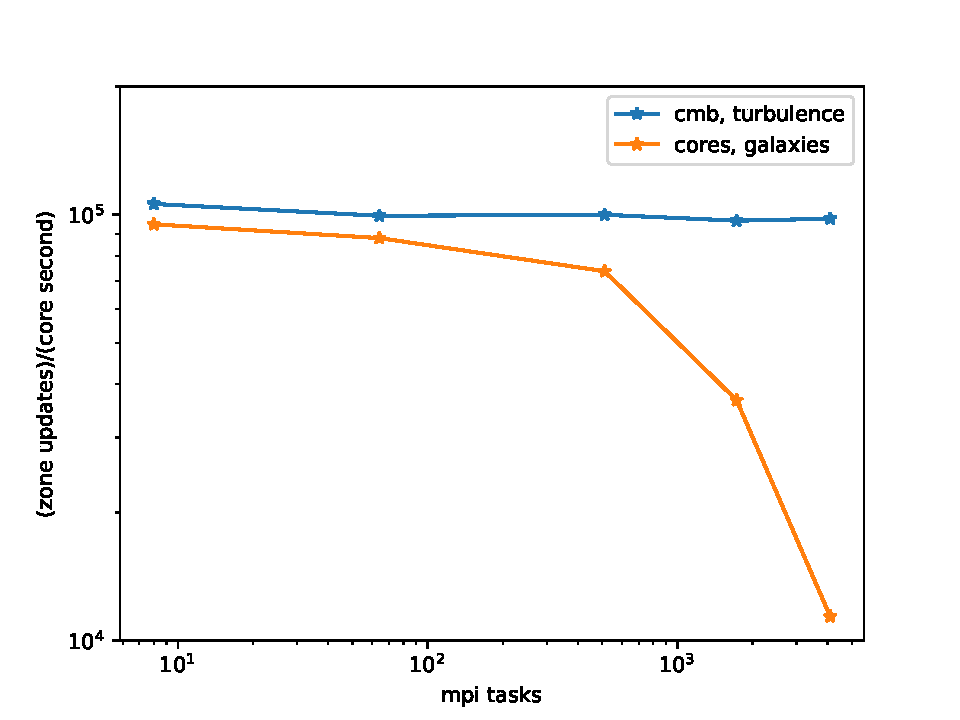
\includegraphics[width=0.99\textwidth]{figs/g49_zoneup.pdf}
\caption[ ]{Zone-pdates per core-second for weak scaling on
    Stampede 2.    
The blue curve only employs
    the MHD solver, in the configuration used for the \nameCMB\ and \nameTurbulence\
    simulations.  The orange curve employs the MHD solver as well as the gravity
    solver and AMR,
 and will be used for the \nameCores\ and \nameGalaxies\ simulations.  The
 gravity and AMR degrade the performance above 512 threads.  This study used 64
 cores per node when possible.}
\label{fig.scaling} \end{center} \end{figure}



\bibliographystyle{apj}
\bibliography{apj-jour,ms.bib}  % looks in ms.bib for bibliography info

\end{document}  


        %dcc todo 2022 
%%\input{SUs}            %dcc todo 2022
%%\input{PriorWork}      %dcc todo 2022 
%%\input{OtherStuff}     %dcc todo 2022

%\appendix
%\include{ appendix file}


\bibliographystyle{apj}
\bibliography{apj-jour,ms}  % looks in ms.bib for bibliography info
%\bibliography{apj-jour,ms}  % looks in ms.bib for bibliography info

\end{document}  


